% !TeX root = ../main.tex
% =============================================================
% Appendix — all sections inlined, no \input{} calls
% =============================================================
\begin{table}[t]
\centering
\caption{Statistics of datasets used in the experiments.}
\renewcommand{\arraystretch}{0.8}
\resizebox{\linewidth}{!}{
\begin{tabular}{c|ccccc}
\toprule
\textbf{Dataset} & \textbf{\#Users} & \textbf{\#Items} & \textbf{\#Interactions} & \textbf{Avg. Length} & \textbf{Sparsity (\%)} \\
\midrule
Toys  & 19,406 & 11,842 & 166,230 & 8.6   & 99.93 \\
Beauty  & 22,363 & 12,077 & 198,064 & 8.9   & 99.93 \\
Sports  & 35,597 & 18,168 & 294,045  & 8.3   & 99.95 \\
Clothing   & 39,387 & 22,445 & 270,319  & 6.9   & 99.97 \\
MovieLens  & 6,040 & 3,397 & 996,867  & 165   & 95.14 \\
\bottomrule
\end{tabular}
}
\label{tab:dataset_stats}
\end{table}
\begin{figure}[!t]
    \centering
    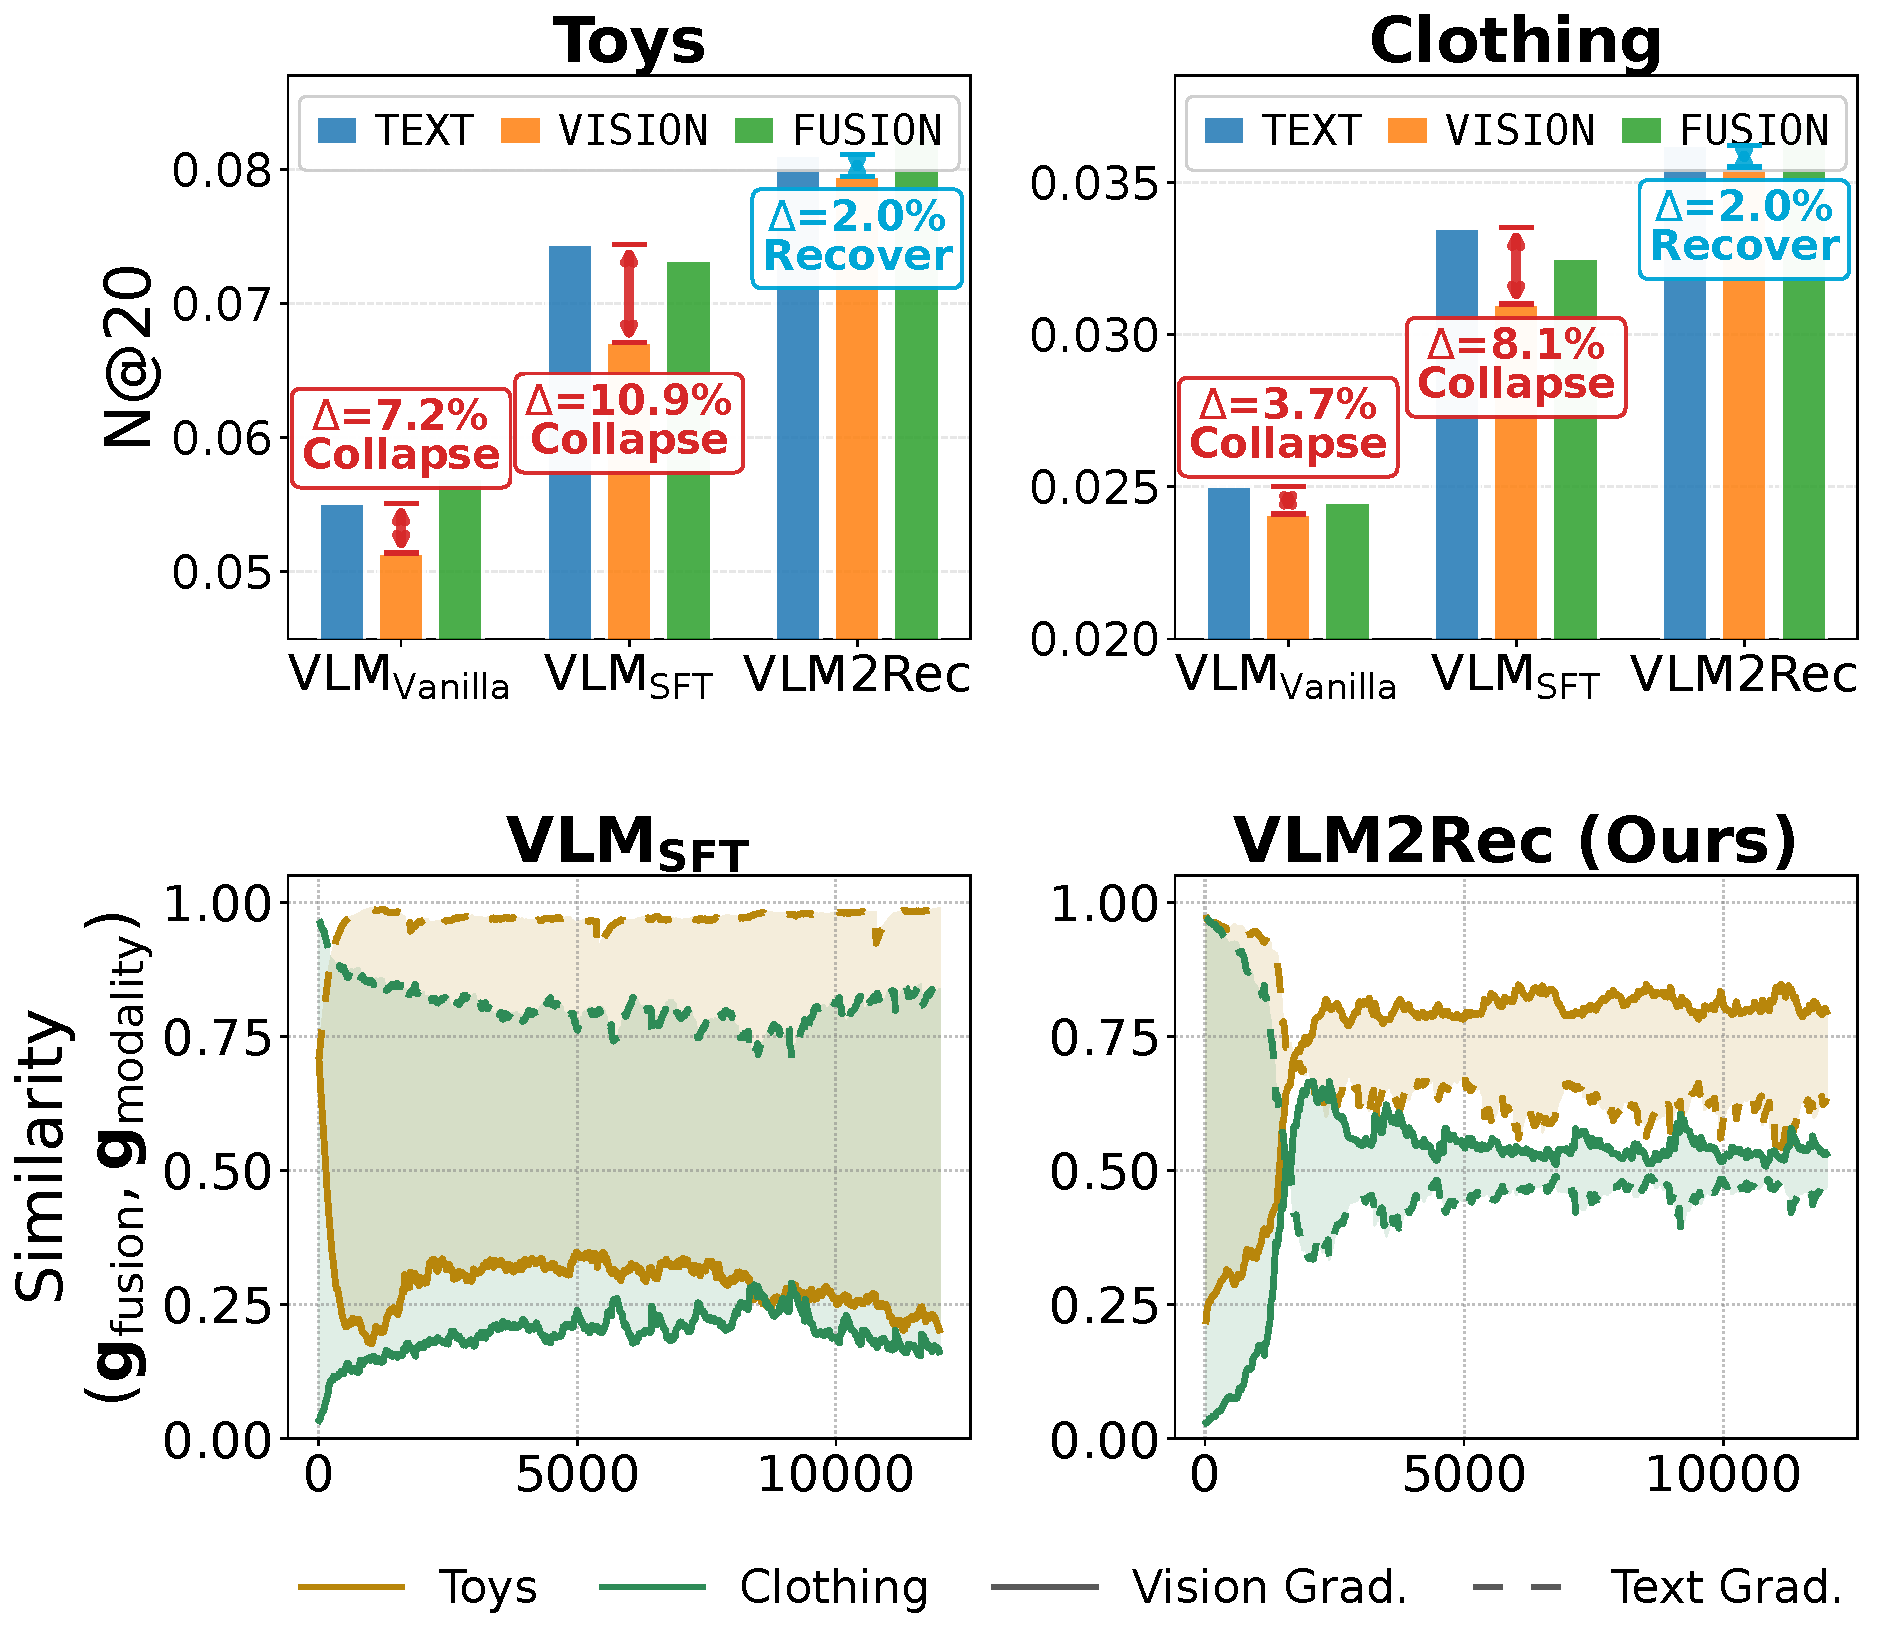
\includegraphics[width=\columnwidth]{figures/drop_grad_Toys_Clothing.pdf}
    \Description{Bar charts compare modality-specific and fused recommendation performance on Toys and Clothing. Line charts show text and vision gradient alignment during SFT and VLM2Rec training.}
    \caption{Modality collapse on Toys and Clothing: dropout test (top) and gradient dynamics (bottom).}
    \label{fig:drop_grad_toys_clothing}
\end{figure}

% ---------------------------------------------------------------

\section{Implementation Details}
\label{app:exp_details}

% \subsection{Implementation Details}
\noindent\textbf{Datasets.}
\label{app:datasets}
We remove items lacking a title or an image (Tab.~\ref{tab:dataset_stats}); for MovieLens, we collect posters from TMDB using the IMDb and TMDB IDs in the MovieLens links file.

\vspace{+0.1cm}
\noindent\textbf{VLM2Rec Pretraining.}
\label{app:implementation_details}
We apply LoRA~\cite{lora} (rank 16, alpha 32, dropout 0.2) and train for 3 epochs with AdamW (learning rate $1\text{e-}5$, batch size 32).
Grid search selects
$\tau_{\text{WPCL}} \in \{0.05, 0.1, 0.5, 1.0\}$,
$\tau_{\text{CRTR}} \in \{0.001, 0.01, 0.1, 1.0\}$, and
$\lambda \in \{0.1, 0.5, 1.0\}$.
With gradient checkpointing, experiments run on one RTX 3090 by default and on one A100 80GB GPU for larger models.

\vspace{+0.1cm}
\noindent\textbf{SR Backbone Training.}
SR backbones are trained on a single RTX 3090 with Adam (learning rate 0.001, $\beta_1=0.9$, $\beta_2=0.999$), batch size 256, dropout 0.5, and early stopping with a patience of 10 epochs on validation N@20.
Baseline hyperparameters are tuned over the search spaces of their original papers.

\vspace{+0.1cm}
\noindent\textbf{Text-based Baselines.}
We use BERT\footnote{google-bert/bert-large-uncased} for text-only item encoding; it embeds items independently, carries no sequence-level CF, and forms sequence representations by mean-pooling its item embeddings.
Following its original paper, SLIM extracts final representations with BERT rather than its student LLM distilled from the ChatGPT API\footnote{gpt-4.1-mini}, so its CF-trained foundation model does not produce the embeddings; our $\text{SLIM}^{+}$ instead extracts them from the student, and both are trained for next-item generation rather than for embedding quality.
LLM2Rec injects sequence-level CF into a text-only LLM embedder, whereas LLMEmb injects CF only indirectly by distilling ID embeddings.
$\text{LLM}_{\text{Vanilla}}$ directly extracts sequence and item embeddings from the foundation model without further training, while $\text{LLM}_{\text{SFT}}$ applies sequence-level contrastive fine-tuning (Eq.~\ref{eq:sft_loss}).

\vspace{+0.1cm}
\noindent\textbf{Multimodal-based Baselines.}
We use CLIP\footnote{openai/clip-vit-large-patch14} for multimodal item encoding, pooled in the same way as BERT.
NoteLLM-2 learns multimodal item embeddings without sequence-level CF, fusing vision through a simple gated sum rather than a dedicated modality-balancing design, and $\text{VLM}_{\text{Prompt}}$ obtains item embeddings by zero-shot prompting without tuning.
I-LLMRec feeds each item's CLIP image feature into a text-only LLM as a single input token, following its original design.
For comparison under the same protocol, we replace the yes/no prediction loss of MLLM-MSR with standard SFT (Eq.~\ref{eq:sft_loss}).
$\text{VLM}_{\text{Vanilla}}$ and $\text{VLM}_{\text{SFT}}$ are the VLM counterparts of $\text{LLM}_{\text{Vanilla}}$ and $\text{LLM}_{\text{SFT}}$; $\text{VLM}_{\text{SFT}}$ thus shares VLM2Rec's backbone, inputs, and CF injection, lacking only modality balancing.

% ---------------------------------------------------------------

% Same layout and size as tables/alignment_uniformity.tex (main-text Tab. ali_uni_clo); values from archive/disabled_geometry.
\begin{table}[!t]
\centering
\caption{VLM geometry on Toys and Clothing: uniformity $U$ and separability $S$.}
\label{tab:ali_uni_toys_clothing}
\setlength{\tabcolsep}{2pt}
\renewcommand{\arraystretch}{0.5}
\resizebox{\columnwidth}{!}{%
\begin{tabular}{@{}lccccccc@{}}
\toprule
\multirow{2}{*}{\textbf{Dataset}} & \multirow{2}{*}{\textbf{Mod.}} & \multicolumn{3}{c}{$U$ ($\downarrow$)} & \multicolumn{3}{c}{$S$ ($\uparrow$)} \\
\cmidrule(lr){3-5}\cmidrule(l){6-8}
 & & $\text{VLM}_{\text{Vanilla}}$ & $\text{VLM}_{\text{SFT}}$ & \textbf{Ours} & $\text{VLM}_{\text{Vanilla}}$ & $\text{VLM}_{\text{SFT}}$ & \textbf{Ours} \\
\midrule
\multirow{3}{*}{\textbf{Toys}}
 & Fused & -0.4707 & -2.2500 & -1.7969 & 1.0609 & 1.2418 & 1.1609 \\
 & Vision & \textbf{-0.0237} & \textcolor{red}{\textbf{-0.0039}} & \textcolor{blue}{\textbf{-0.5703}} & \textbf{1.0039} & \textcolor{red}{\textbf{0.9911}} & \textcolor{blue}{\textbf{1.1551}} \\
 & Text & -0.4453 & -2.2188 & -0.9335 & 1.0673 & 1.2480 & 1.1218 \\
\midrule
\multirow{3}{*}{\textbf{Clothing}}
 & Fused & -0.4336 & -1.8359 & -1.9951 & 1.0444 & 1.0474 & 1.1274 \\
 & Vision & \textbf{-0.2368} & \textcolor{red}{\textbf{-0.0237}} & \textcolor{blue}{\textbf{-1.2136}} & \textbf{1.0110} & \textcolor{red}{\textbf{0.9997}} & \textcolor{blue}{\textbf{1.0706}} \\
 & Text & -0.4102 & -1.7187 & -1.3759 & 1.0551 & 1.0562 & 1.0610 \\
\bottomrule
\end{tabular}%
}
\end{table}

\begin{table}[!t]
\centering
\caption{Frozen-VLM Head-SFT control in the $\text{VLM2Rec}_{\text{plug}}$ setting (SASRec, N@20).}
\label{tab:head_sft_control}
% \footnotesize
\setlength{\tabcolsep}{3pt}
\renewcommand{\arraystretch}{0.8}
\begin{tabular*}{\columnwidth}{@{\extracolsep{\fill}}llcccc@{}}
\toprule
\textbf{Dataset} & \textbf{Variant} & \textbf{\TEXTset} & \textbf{\VISIONset} & \textbf{\FUSIONset} & \textbf{Gap} (\%) \\
\midrule
\multirow{3}{*}{Beauty}
 & $\text{VLM}_{\text{Vanilla}}$ & 0.0469 & 0.0438 & 0.0463 & 7.08 \\
 & Head-SFT    & 0.0467 & 0.0385 & 0.0462 & 21.30 \\
 & $\text{VLM}_{\text{SFT}}$     & 0.0650 & 0.0587 & 0.0622 & 10.73 \\
\midrule
\multirow{3}{*}{MovieLens}
 & $\text{VLM}_{\text{Vanilla}}$ & 0.0665 & 0.0622 & 0.0695 & 6.91 \\
 & Head-SFT    & 0.0950 & 0.0751 & 0.0916 & 26.50 \\
 & $\text{VLM}_{\text{SFT}}$     & 0.1100 & 0.0953 & 0.1082 & 15.42 \\
\bottomrule
\end{tabular*}
\end{table}

\section{Additional Analysis}
\label{app:additional_empirical_analyses}

% ---------------------------------------------------------------
\subsection{Modality-collapse Analyses}
% ---------------------------------------------------------------

\noindent\textbf{Additional Domains.}
\label{app:additional_analysis}
Standard SFT again biases the fused update toward the stronger modality and widens the \TEXTset{}--\VISIONset{} gap on Toys and on Clothing (Fig.~\ref{fig:drop_grad_toys_clothing}), so the pattern holds even in the visually informative Clothing domain.
The geometry repeats the pattern of Tab.~\ref{tab:ali_uni_clo} (Tab.~\ref{tab:ali_uni_toys_clothing}): $\text{VLM}_{\text{SFT}}$ keeps visual separability $S$ at or below the discrimination threshold and degrades visual uniformity $U$, whereas VLM2Rec restores both, balances the gradients, and lets \FUSIONset{} surpass either single-modality input, consistent with Sec.~\ref{sec:modality_mute}.

% defined before B.2, which cites it
\begin{table}[!t]
\centering
\caption{Performance on additional SR backbones (N@20). \protect\colorbox{bestcolor}{\textbf{Bold}}/\protect\colorbox{secondcolor}{\underline{underline}}: best/second best; *: $p<0.05$ (paired $t$-test, 5 seeds).}
\setlength{\tabcolsep}{3pt}
\resizebox{\columnwidth}{!}{
\renewcommand{\arraystretch}{0.8}
\begin{tabular}{c|cc|cccc|cc}
\toprule
\multirow{2}{*}{\textbf{Data}} & \multicolumn{2}{c|}{\textbf{Text-based Models}} & \multicolumn{4}{c|}{\textbf{Multimodal-based Models}} & \multicolumn{2}{c}{\textbf{Ours}} \\
\cmidrule(lr){2-3} \cmidrule(lr){4-7} \cmidrule(lr){8-9}
 & LLM2Rec & $\text{LLM}_{\text{SFT}}$ & $\text{VLM}_{\text{Van}}$ & $\text{VLM}_{\text{SFT}}$ & MLLM-MSR & I-LLMRec & \textbf{$\text{VLM2Rec}_{\text{plug}}$} & \textit{Imp(\%)} \\ \midrule

\midrule[\heavyrulewidth]
\multicolumn{9}{c}{\cellcolor{gray!15}\textbf{Backbone: DiffuRec}} \\ \midrule

\textbf{Toys} & 0.0639 & 0.0644 & 0.0586 & 0.0655 & 0.0650 & \secondscore{0.0658} & \bestscore{0.0760*} & 15.50 \\

\textbf{Beauty} & 0.0656 & 0.0670 & 0.0561 & 0.0682 & 0.0674 & \secondscore{0.0689} & \bestscore{0.0740*} & 7.40 \\

\textbf{Clothing} & 0.0316 & 0.0325 & 0.0291 & \secondscore{0.0334} & 0.0323 & 0.0327 & \bestscore{0.0384*} & 14.97 \\

\textbf{Sports} & 0.0319 & 0.0334 & 0.0288 & 0.0322 & 0.0340 & \secondscore{0.0347} & \bestscore{0.0398*} & 14.70 \\

\textbf{MovieLens} & 0.1036 & 0.1071 & 0.0767 & 0.1096 & 0.1077 & \secondscore{0.1112} & \bestscore{0.1188*} & 6.83 \\
\midrule[\heavyrulewidth]
\multicolumn{9}{c}{\cellcolor{gray!15}\textbf{Backbone: FMLP}} \\ \midrule

\textbf{Toys} & 0.0639 & 0.0660 & 0.0534 & 0.0642 & 0.0664 & \secondscore{0.0670} & \bestscore{0.0732*} & 9.25 \\

\textbf{Beauty} & 0.0552 & 0.0564 & 0.0432 & 0.0585 & 0.0569 & \secondscore{0.0598} & \bestscore{0.0691*} & 15.55 \\

\textbf{Clothing} & 0.0265 & 0.0269 & 0.0206 & 0.0281 & 0.0264 & \secondscore{0.0285} & \bestscore{0.0341*} & 19.65 \\

\textbf{Sports} & 0.0272 & 0.0278 & 0.0225 & 0.0284 & 0.0280 & \secondscore{0.0285} & \bestscore{0.0353*} & 23.86 \\

\textbf{MovieLens} & 0.0844 & 0.0867 & 0.0582 & \secondscore{0.0913} & 0.0876 & 0.0909 & \bestscore{0.1057*} & 15.77 \\
\midrule[\heavyrulewidth]
\multicolumn{9}{c}{\cellcolor{gray!15}\textbf{Backbone: GRU4Rec}} \\ \midrule

\textbf{Toys} & 0.0447 & 0.0454 & 0.0424 & 0.0465 & 0.0463 & \secondscore{0.0475} & \bestscore{0.0576*} & 21.26 \\

\textbf{Beauty} & 0.0470 & 0.0476 & 0.0422 & 0.0485 & 0.0478 & \secondscore{0.0491} & \bestscore{0.0548*} & 11.61 \\

\textbf{Clothing} & 0.0231 & 0.0233 & 0.0204 & \secondscore{0.0242} & 0.0231 & 0.0239 & \bestscore{0.0264*} & 9.09 \\

\textbf{Sports} & 0.0267 & 0.0279 & 0.0216 & 0.0273 & 0.0283 & \secondscore{0.0289} & \bestscore{0.0305*} & 5.54 \\

\textbf{MovieLens} & 0.0829 & 0.0867 & 0.0587 & \secondscore{0.0902} & 0.0876 & 0.0896 & \bestscore{0.0965*} & 6.98 \\\bottomrule

 \end{tabular}
}
\label{tab:add_backbones}
\end{table}

\noindent\textbf{Analysis of the SFT Objective.}
\label{app:head_sft_control}
Fused contrastive SFT can amplify modality collapse with a frozen VLM (Tab.~\ref{tab:head_sft_control}).
To separate its effect from LoRA updates (Fig.~\ref{fig:drop_grad}), we train only a linear head with the same loss (Head-SFT), then evaluate the item embeddings with SASRec in the $\text{VLM2Rec}_{\text{plug}}$ setting.
The \TEXTset{}--\VISIONset{} gap widens beyond that of $\text{VLM}_{\text{Vanilla}}$ on both datasets, and head-only gradients remain text-dominant.

% ---------------------------------------------------------------
\subsection{Robustness and Efficiency}
% ---------------------------------------------------------------

\noindent\textbf{Additional Backbone Results.}
\label{sec:add_backbone}
$\text{VLM2Rec}_{\text{plug}}$ performs best on the diffusion-based DiffuRec~\cite{diffurec}, the MLP-based FMLP~\cite{fmlp}, and the RNN-based GRU4Rec~\cite{gru4rec} (Tab.~\ref{tab:add_backbones}), indicating that its embeddings transfer across architectures.

\begin{table}[!htb]
\centering
\caption{Modality dropout test across VLM backbones (Beauty, SASRec, N@20).}
\label{tab:modality_collapse_backbones}
\setlength{\tabcolsep}{2.5pt}
\resizebox{\columnwidth}{!}{
\renewcommand{\arraystretch}{0.8}
\begin{tabular}{l|ccc|c|ccc|c}
\toprule
\multirow{2}{*}{\textbf{VLM Backbone}}
 & \multicolumn{4}{c|}{\textbf{$\text{VLM}_{\text{SFT}}$}}
 & \multicolumn{4}{c}{\textbf{VLM2Rec}} \\
\cmidrule(lr){2-5} \cmidrule(lr){6-9}
 & \TEXTset{} & \VISIONset{} & \FUSIONset{} & \textbf{Gap (\%)}
 & \TEXTset{} & \VISIONset{} & \FUSIONset{} & \textbf{Gap (\%)} \\
\midrule
InternVL3-2B    & 0.0614 & 0.0558 & 0.0608 & 10.04 & 0.0703 & 0.0686 & 0.0702 & \textbf{2.48} \\
Qwen2.5-VL-7B   & 0.0636 & 0.0588 & 0.0632 &  8.16 & 0.0746 & 0.0733 & 0.0754 & \textbf{1.77} \\
LLaVA-1.5-7B    & 0.0625 & 0.0572 & 0.0620 &  9.27 & 0.0733 & 0.0725 & 0.0742 & \textbf{1.10} \\
InternVL3-8B    & 0.0645 & 0.0597 & 0.0636 &  8.04 & 0.0744 & 0.0727 & 0.0750 & \textbf{2.34} \\
Qwen2.5-VL-32B  & 0.0653 & 0.0612 & 0.0647 &  6.70 & 0.0761 & 0.0744 & 0.0776 & \textbf{2.28} \\
\bottomrule
\end{tabular}
}
\end{table}

\begin{figure}[!htb]
    \centering
    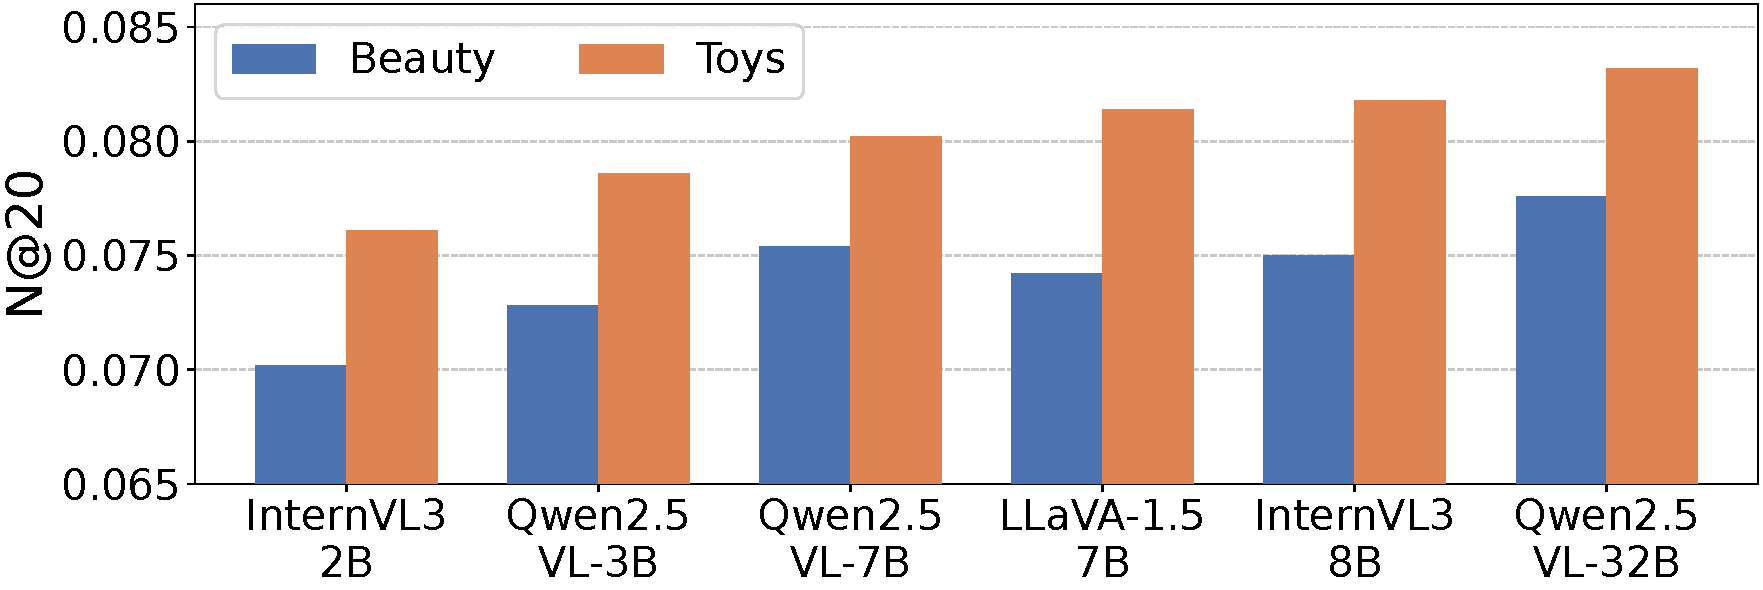
\includegraphics[width=\columnwidth]{figures/model_scalability.pdf}
    \Description{Grouped bars compare VLM2Rec's N@20 on Beauty and Toys for six VLM backbones from three families, ranging from two billion to thirty-two billion parameters.}
    \caption{Model scalability across VLM families and parameter sizes (SASRec, N@20).}
    \label{fig:model_capacity}
\end{figure}

\noindent\textbf{VLM Backbones and Scalability.}
\label{app:modality_collapse_backbones}
\label{app:model_scalability}
We rerun the modality dropout test on Beauty across five backbones spanning three model families (InternVL3~\cite{internvl3}, Qwen2.5-VL~\cite{qwen2.5-vl}, LLaVA-1.5~\cite{llava}) and four scales (2B--32B) (Tab.~\ref{tab:modality_collapse_backbones}).
For every backbone, $\text{VLM}_{\text{SFT}}$ shows a sizable \TEXTset{}--\VISIONset{} gap, which VLM2Rec substantially narrows while improving \FUSIONset{}, so the SFT-amplified collapse and its mitigation are not artifacts of a specific backbone.
VLM2Rec's recommendation performance also scales with model capacity on both Beauty and Toys, while models of similar size perform comparably across families (Fig.~\ref{fig:model_capacity}), so the model size can follow deployment budgets.

\begin{table}[!h]
\centering
\caption{VLM2Rec on Qwen3-VL-Embedding in the $\text{VLM2Rec}_{\text{plug}}$ setting (SASRec, N@20). Base: the released model without our training. Gap: (\TEXTset{}$-$\VISIONset{})/\VISIONset{}; lower is better.}
\label{tab:qwen3_vl_embedding}
% \footnotesize
\setlength{\tabcolsep}{7pt}
\renewcommand{\arraystretch}{0.5}
\resizebox{\linewidth}{!}{%
\begin{tabular}{lllcccc}
\toprule
\textbf{Data} & \textbf{Size} & \textbf{Variant} & \textbf{\TEXTset} & \textbf{\VISIONset} & \textbf{\FUSIONset} & \textbf{Gap (\%)} \\
\midrule
Beauty & 2B & Base & 0.0732 & 0.0672 & 0.0719 & 8.93 \\
       &    & +VLM2Rec & 0.0751 & 0.0718 & 0.0746 & 4.60 \\
       & 8B & Base & 0.0745 & 0.0692 & 0.0729 & 7.66 \\
       &    & +VLM2Rec & 0.0762 & 0.0734 & 0.0751 & 3.81 \\
\midrule
MovieLens & 2B & Base & 0.1176 & 0.1034 & 0.1147 & 13.73 \\
          &    & +VLM2Rec & 0.1179 & 0.1098 & 0.1162 & 7.38 \\
          & 8B & Base & 0.1211 & 0.1119 & 0.1186 & 8.22 \\
          &    & +VLM2Rec & 0.1206 & 0.1187 & 0.1192 & 1.60 \\
\bottomrule
\end{tabular}%
}
\end{table}

\noindent\textbf{Pretrained Multimodal Embedders.}
\label{app:embedding_vlm_transfer}
We apply VLM2Rec to the open-source Qwen3-VL-Embedding 2B and 8B models~\cite{qwen3_vl_embedding}, already trained on large-scale multimodal retrieval tasks, on Beauty and MovieLens (Tab.~\ref{tab:qwen3_vl_embedding}).
Even these embedders show a sizable \TEXTset{}--\VISIONset{} gap (7.7--13.7\%).
Within each backbone, VLM2Rec substantially reduces the \TEXTset{}--\VISIONset{} gap and increases fused N@20 in all four comparisons, with the largest gains in vision-only ranking; text-only performance is not uniformly higher (e.g., the 8B MovieLens case).
These within-backbone results show that weak-modality correction also benefits pretrained multimodal embedders; we compare only within each backbone, since these embedders are trained at a far larger scale than the models in Tab.~\ref{tab:perf_task2}.

\begin{table}[!h]
\centering
% \small
\caption{Time and space complexity of the loss objectives.}
\renewcommand{\arraystretch}{0.8}
\setlength{\tabcolsep}{3pt}
\resizebox{\columnwidth}{!}{%
\begin{tabular}{lcccc}
\toprule
\textbf{Objective} & \textbf{Time} & \textbf{Space} & \textbf{In-batch Time} & \textbf{In-batch Space} \\
\midrule
$\mathcal{L}_{\text{SFT}}$
& $O\!\left(2B(N{+}1)d\right)$
& $O\!\left(B(N{+}1)\right)$
& $O(2B^2d)$
& $O(B^2)$ \\
$\mathcal{L}_{\text{WPCL}}$
& $O\!\left(6B(N{+}1)d\right)$
& $O\!\left(B(N{+}1)\right)$
& $O(6B^2d)$
& $O(B^2)$ \\
$\mathcal{L}_{\text{CRTR}}$
& $O(4BCd)$
& $O(BC)$
& $O(4B^2d)$
& $O(B^2)$ \\
\bottomrule
\end{tabular}%
}
\label{tab:complexity_loss}
\end{table}

\noindent\textbf{Computational Complexity.}
\label{app:complexity}
Tab.~\ref{tab:complexity_loss} compares the loss computation after backbone encoding, where $B = |\mathcal{B}|$ is the batch size, $N=|\mathcal{N}_u|$ the number of negatives per user, $C=|\mathcal{C}|$ the candidate set size of $\mathcal{L}_{\text{CRTR}}$, and $d$ the embedding dimension; space denotes the additional memory of the loss computation, excluding backbone activations.
$\mathcal{L}_{\text{WPCL}}$ adds two modality-wise similarity passes to $\mathcal{L}_{\text{SFT}}$ with the same space, and $\mathcal{L}_{\text{CRTR}}$ builds modality-wise sequence-to-candidate similarity matrices.
With in-batch negatives and candidates ($N=B-1$, $|\mathcal{C}|=B$), all three losses cost $O(B^2d)$ time and $O(B^2)$ space, differing only in constant factors.

\begin{table}[t]
\centering
\caption{Item embedding generation time (sec), measured once per catalog.}
\label{tab:emb_time}
\setlength{\tabcolsep}{3pt}
\resizebox{\columnwidth}{!}{
\renewcommand{\arraystretch}{0.7}
\begin{tabular}{l|cccccc|c}
\toprule
\textbf{Dataset} & LLMEmb & LLM2Rec & $\text{LLM}_{\text{SFT}}$ & NoteLLM-2 & $\text{VLM}_{\text{SFT}}$ & I-LLMRec & $\text{VLM2Rec}_{\text{plug}}$ \\
\midrule
Beauty & 58 & 58 & 56 & 132 & 113 & 60 & 113 \\
Toys & 38 & 39 & 39 & 91 & 79 & 41 & 79 \\
\bottomrule
\end{tabular}
}
\end{table}

\vspace{+0.1cm}
\noindent\textbf{Item Embedding Generation Time.}
\label{app:emb_time}
Tab.~\ref{tab:emb_time} reports the time to encode each catalog once, complementing the training times in Fig.~\ref{fig:few_shot}.
$\text{VLM2Rec}_{\text{plug}}$ takes the same time as $\text{VLM}_{\text{SFT}}$ for every $K_u$, since both encode titles and images with the same VLM.

\begin{table}[t]

\centering
\caption{Effect of negative sampling strategies for $\Delta_{u,\mathrm{gap}}$ estimation (SASRec, N@20).}
\label{tab:negative_sampling}
\resizebox{\linewidth}{!}{
\renewcommand{\arraystretch}{0.7}
\begin{tabular}{l|ccccc}
\toprule
\textbf{Dataset} & \textbf{In-batch} & \textbf{Random} & \textbf{SASRec Top-$k$} & \textbf{Text Sim.} & \textbf{Image Sim.} \\
\midrule
Clothing & 0.0345 & 0.0342 & 0.0352 & 0.0357 & 0.0360 \\
MovieLens    & 0.1216 & 0.1193 & 0.1218 & 0.1222 & 0.1229 \\
\bottomrule
\end{tabular}
}

\end{table}

\vspace{+0.1cm}
\noindent\textbf{Negative Sampling for $\Delta_{u,\mathrm{gap}}$ Estimation.}
\label{app:negative_sampling}
Harder negatives for estimating $\Delta_{u,\text{gap}}$ (Eq.~\ref{eq:modality_gap}) improve N@20 over the in-batch negatives of our main experiments (Tab.~\ref{tab:negative_sampling}).
SASRec Top-$k$ uses each user's top-$k$ SASRec predictions, while Text Sim. and Image Sim. sample target-similar items by BERT and CLIP similarity, respectively.
Image-similar negatives perform best, suggesting that fine-grained visual distinctions sharpen the $\Delta_{u,\mathrm{gap}}$ estimate for the weak visual modality; we keep in-batch negatives to avoid retrieval cost, while modality-aware hard negatives could help further.

\begin{figure}[!h]
    \centering
    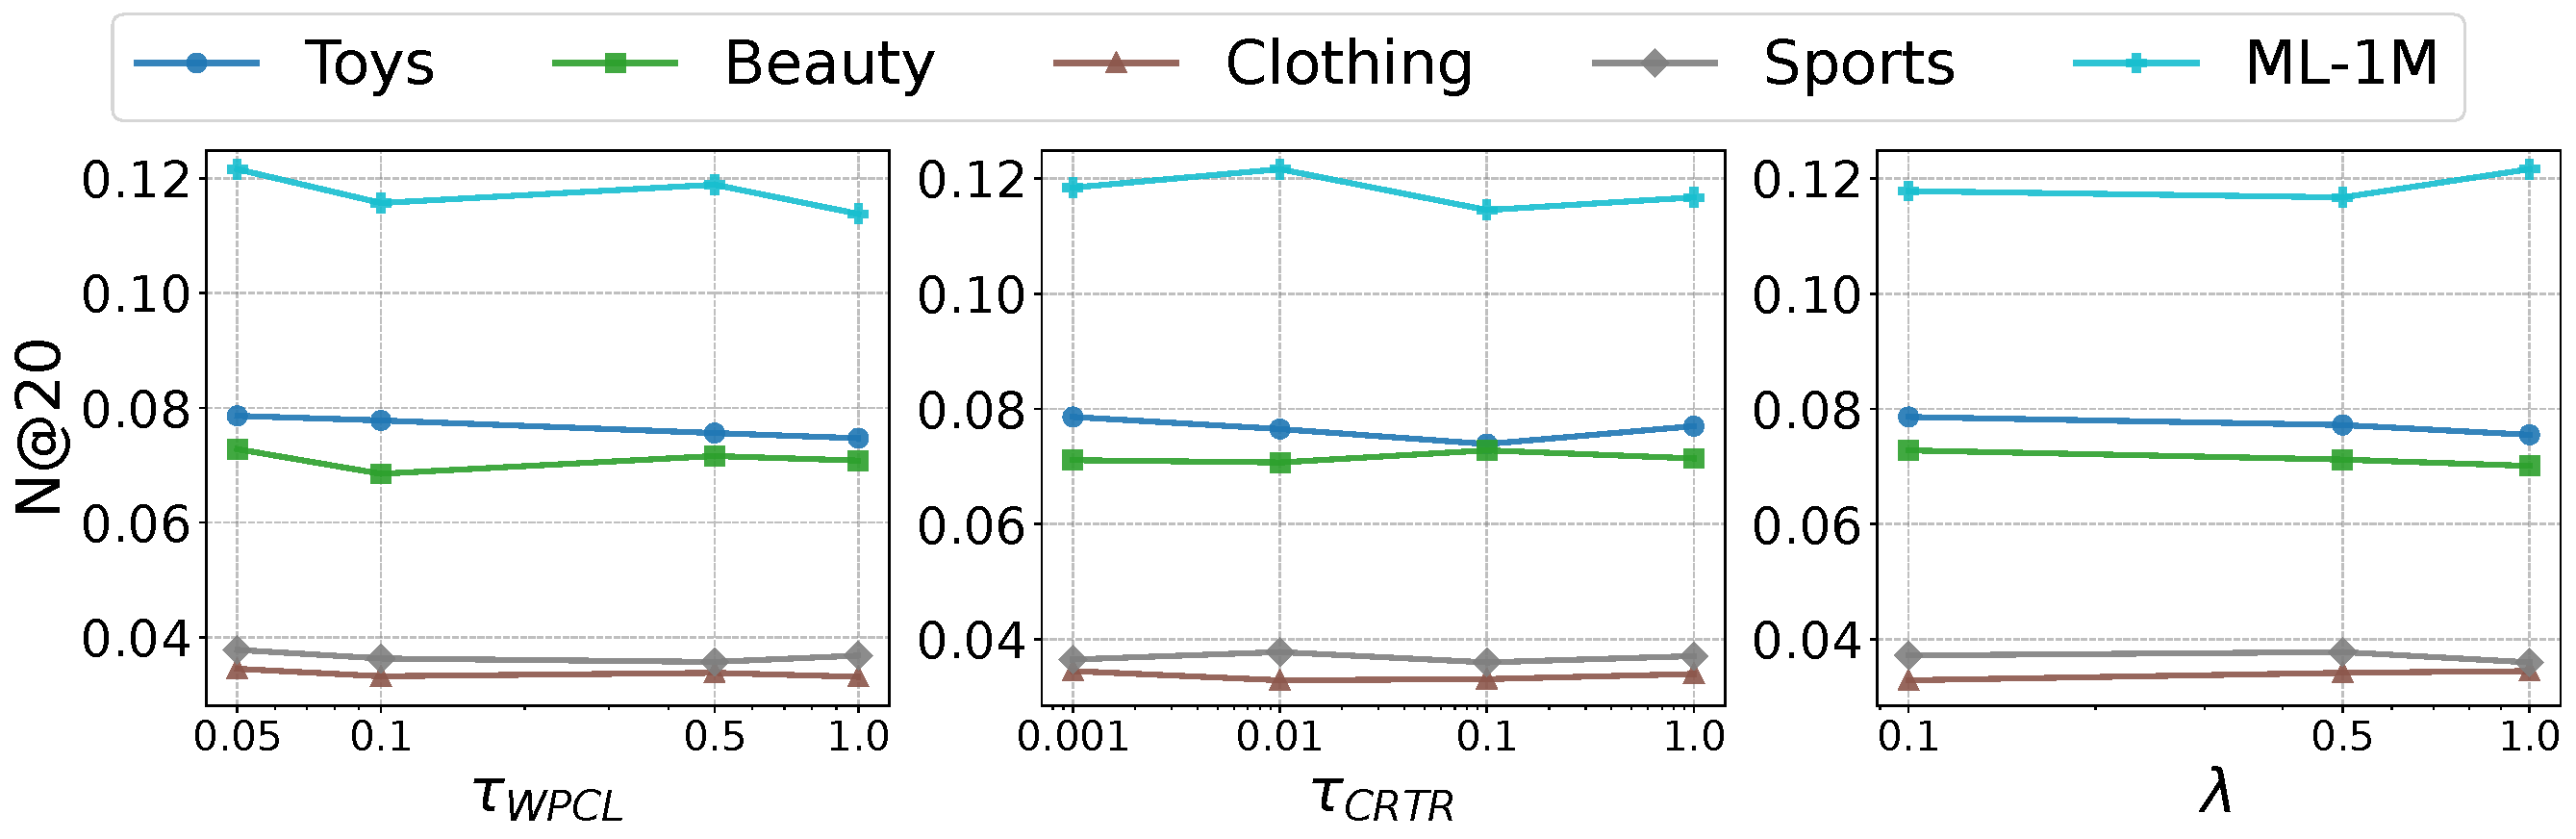
\includegraphics[width=\linewidth]{figures/hyperparameter.pdf}
    \Description{Three line plots show VLM2Rec-plug N@20 with SASRec on five datasets as the WPCL temperature, CRTR temperature, and regularization weight vary.}
    \caption{Hyperparameter study of $\text{VLM2Rec}_{\text{plug}}$ (SASRec, N@20).}
    \label{fig:hyperparameter}
\end{figure}

\noindent\textbf{Hyperparameter Study.}
\label{app:hyperparameter}
Across the tested settings, N@20 varies little and stays above the baselines (Fig.~\ref{fig:hyperparameter}).
This limits the tuning cost of $\text{VLM2Rec}_{\text{plug}}$.

% ---------------------------------------------------------------
\subsection{User-level Analysis}
% ---------------------------------------------------------------

\begin{table}[!t]
\centering
\caption{Anchor weak-modality split. Ratio: fraction of users whose anchor weak modality is text or vision.}
\label{tab:user_anchor_split}
\resizebox{\linewidth}{!}{
\renewcommand{\arraystretch}{0.7}
\begin{tabular}{lllcccc}
\toprule
\textbf{Data} & \textbf{Group} & \textbf{Weak} & \textbf{Ratio} & \textbf{$\Delta_{u,\mathrm{gap}}^{\text{SFT}}$} & \textbf{$\Delta_{u,\mathrm{gap}}^{\text{Ours}}$} & \textbf{User Red.} \\
\midrule
\multirow{4}{*}{MovieLens}
 & \multirow{2}{*}{All}      & Text   & 0.2728 & 0.2864 & 0.0235 & 0.9064 \\
 &                            & Vision & 0.7272 & 0.4047 & 0.0639 & 0.9473 \\
\cmidrule(lr){2-7}
 & \multirow{2}{*}{Collapse} & Text   & 0.2090 & 0.5563 & 0.0250 & 1.0000 \\
 &                            & Vision & 0.7910 & 0.6522 & 0.0808 & 1.0000 \\
\midrule
\multirow{4}{*}{Clothing}
 & \multirow{2}{*}{All}      & Text   & 0.4621 & 0.1346 & 0.0201 & 0.8224 \\
 &                            & Vision & 0.5379 & 0.1467 & 0.0232 & 0.8326 \\
\cmidrule(lr){2-7}
 & \multirow{2}{*}{Collapse} & Text   & 0.4891 & 0.2797 & 0.0529 & 0.9923 \\
 &                            & Vision & 0.5109 & 0.2803 & 0.0592 & 0.9932 \\
\bottomrule
\end{tabular}
}
\end{table}

\noindent\textbf{Anchor Weak-modality Analysis.}
\label{app:anchor_weak_split}
We split each user group by the anchor weak modality, the weaker modality under $\text{VLM}_{\text{Vanilla}}$; \textit{All} and \textit{Collapse} follow Sec.~\ref{sec:user_stratification}.
Vision is the weak modality for most users on both datasets (Tab.~\ref{tab:user_anchor_split}), consistent with the text dominance of VLMs, although its share drops on the visually rich Clothing.
VLM2Rec substantially lowers the gap from $\Delta_{u,\mathrm{gap}}^{\text{SFT}}$ to $\Delta_{u,\mathrm{gap}}^{\text{Ours}}$ in every split, and most users show $\Delta_{u,\mathrm{gap}}^{\text{Ours}}<\Delta_{u,\mathrm{gap}}^{\text{SFT}}$ (\textit{User Red.}), confirming recovery for both text-weak and vision-weak users.

\begin{figure}[!t]
    \centering
    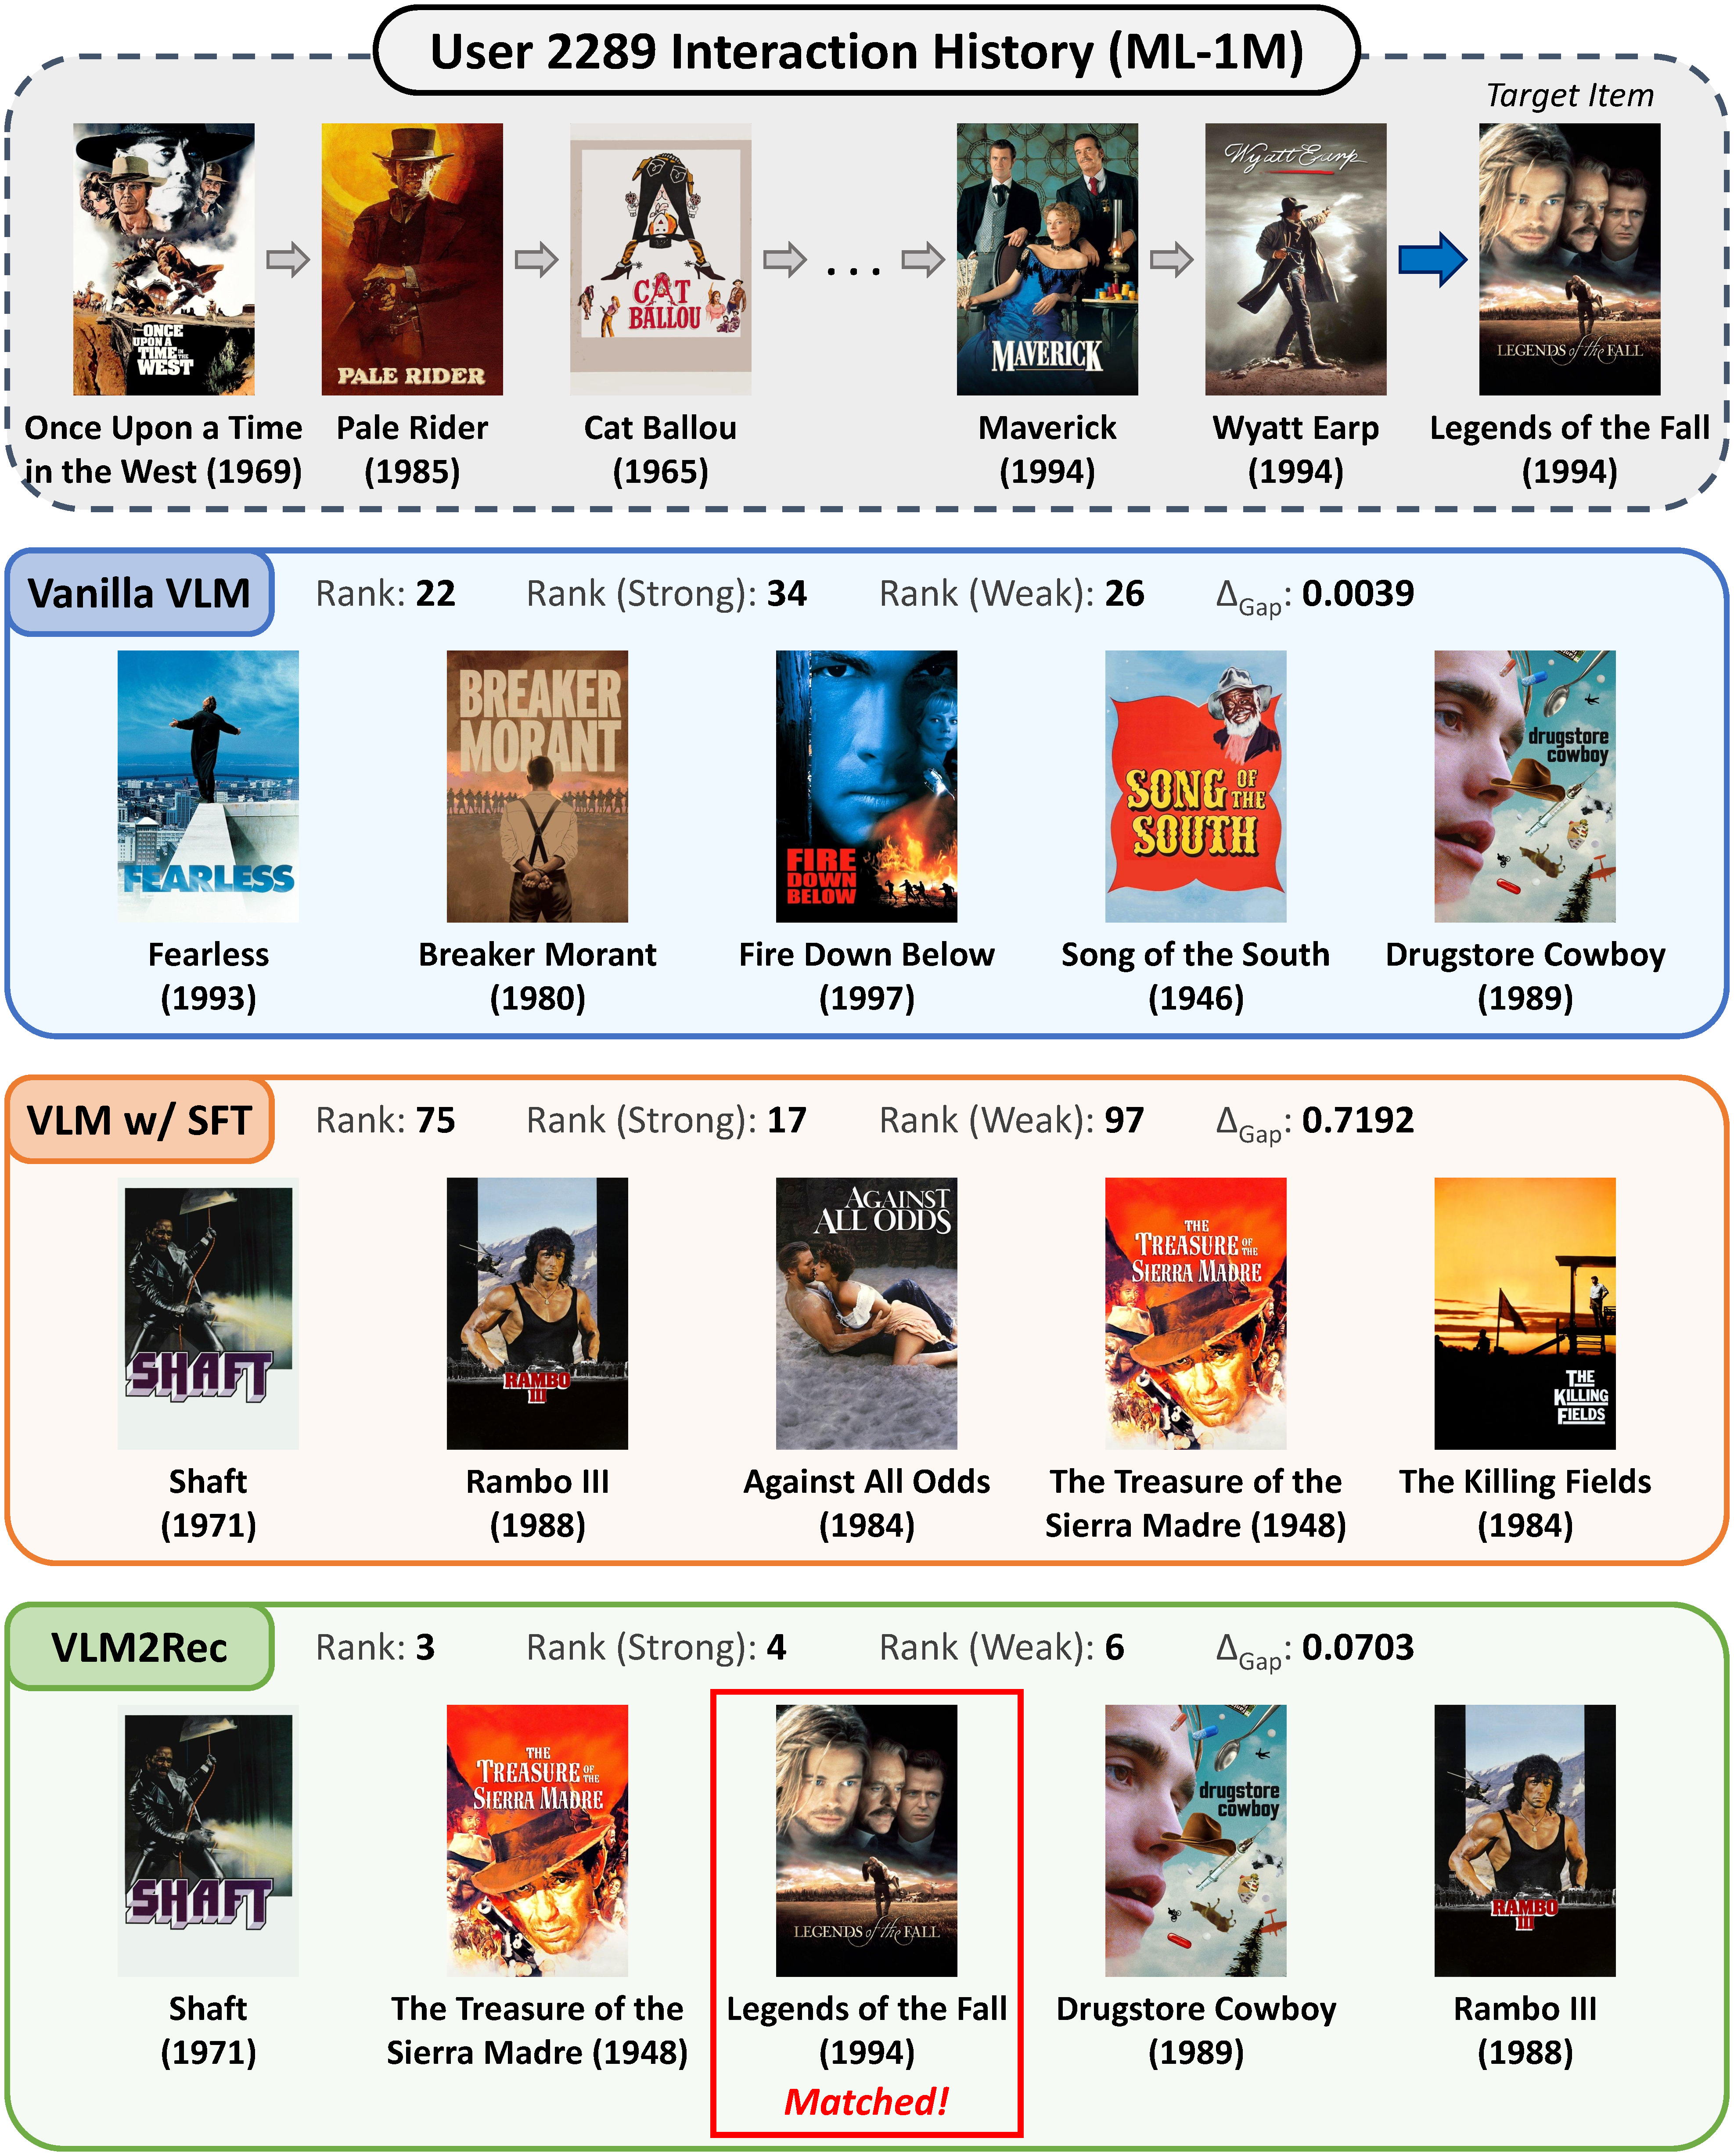
\includegraphics[width=\columnwidth]{figures/case_study.pdf}
    \Description{A MovieLens user history and target movie are followed by the top five recommendations from vanilla VLM, SFT, and VLM2Rec. The target rank worsens after SFT and improves with VLM2Rec.}
    \caption{Case study: Top-5 prediction lists of each model.}
    \label{fig:case_study}
\end{figure}

\vspace{+0.1cm}
\noindent\textbf{Case Study.}
\label{app:case_study}
For a \textit{Collapse} user (Sec.~\ref{sec:user_stratification}; Fig.~\ref{fig:case_study}), $\text{VLM}_{\text{SFT}}$'s recommendations are dominated by the stronger modality, illustrating how the weak-modality signal can be suppressed even after CF supervision is injected.
VLM2Rec instead recovers a more balanced multimodal representation and ranks candidates that better reflect the target preference, showing how weak-modality recovery translates into an individual recommendation.

% Proofs removed with the theoretical analysis (2026-10-26; kept for reference).
% % ---------------------------------------------------------------
% \section{Proofs}
% \label{app:proofs}
% % ---------------------------------------------------------------

% \subsection{Proof of \texorpdfstring{Proposition~\ref{prop:wpcl}}{the WPCL proposition}}
% \label{app:proof_wpcl}
% \begin{proof}
% (i) Since $\partial\ell_u/\partial w_{u,\text{pen}}=B_u/(A_u+w_{u,\text{pen}}B_u)$ and $\mathrm{sg}[\cdot]$ detaches the strong margin, the chain rule through Eq.~\ref{eq:wpen} gives $\gamma_u=\sigma(\Delta_{u,\mathrm{gap}})\,B_u/(A_u+w_{u,\text{pen}}B_u)$, where $\sigma$ is the sigmoid.
% (ii) Rewriting Eq.~\ref{eq:wpcl} gives
% \begin{equation}
% \ell_u=\mathrm{Softplus}\!\left(\frac{r_u^--s_u^+}{\tau_{\text{WPCL}}}+\log w_{u,\text{pen}}\right),
% \label{eq:wpcl_multineg_theory}
% \end{equation}
% so $\ell_u\le c$ exactly when $s_u^+-r_u^-$ is at least $\tau_{\text{WPCL}}\log w_{u,\text{pen}}$ plus a constant that depends only on $c$; $w_{u,\text{pen}}$ increases with $\Delta_{u,\mathrm{gap}}$.
% \end{proof}

% \subsection{Proof of \texorpdfstring{Proposition~\ref{prop:crtr}}{the CRTR proposition}}
% \label{app:proof_crtr}
% \begin{proof}
% (i) KL is nonnegative and vanishes only for identical distributions, so $D_u=0$ exactly when $\mathbf P^T_u=\mathbf P^V_u$, i.e., when the two softmax logits differ by a constant: $s^T_{u,j}-s^V_{u,j}$ is constant over $j\in\mathcal{C}$.
% (ii) Cosine similarity is invariant to such maps; applying an orthogonal $\mathbf Q$ with $\mathbf Q\mathbf e^T_u\neq\mathbf e^T_u$ to the vision embeddings of a configuration with identical text and vision embeddings keeps $D_u=0$ but gives $\mathbf e^V_u\neq\mathbf e^T_u$.
% (iii) Summing Pinsker's inequality, $\mathrm{KL}\ge\frac{1}{2}\|\mathbf P^T_u-\mathbf P^V_u\|_1^2$ (natural logarithm), over the two terms gives the bound.
% \end{proof}

\clearpage
